\documentclass{article}

\usepackage{fullpage,amsmath,amsthm,graphicx,enumitem}
\usepackage{hyperref}
\usepackage{amssymb}
\usepackage{wasysym}
\usepackage{empheq}
\usepackage{siunitx}

%For Grid, thanks internet: https://tex.stackexchange.com/questions/247541/help-with-grid-lines-in-a-pgfplot
\usepackage{tikz}
\usepackage{pgfplots}
\usetikzlibrary{calc}
\newcommand{\comment}[1]{\textcolor{blue}{[Comment: #1]}}

\theoremstyle{definition}
\newtheorem{question}{Question}

\newcommand{\option}{{\Large$\Square$ }}

\title{ASEN 3728 Aircraft Dynamics\\Written Homework 6}

\date{Due date listed on Gradescope.}

\begin{document}

\maketitle

\begin{question} TRUE or FALSE and Justify:
    \begin{enumerate}
        \item Consider an aircraft designed with typical stabilizing dihedral effect. If the wind that this aircraft is flying into suddenly changes so that the sideslip angle $\beta$ suddenly becomes positive, the immediate reaction of the aircraft in the roll direction will be a positive roll ($p > 0$) into the wind.

        \item Consider an aircraft that is designed to be statically stable. The sign of the stability derivative $C_{l_p}$ is negative.

        \item Consider a typical aircraft with the center of gravity of the vertical tail being located above and behind the center of gravity of the entire aircraft. If the aircraft is suddenly hit by a gust of wind such that it now has a positive yaw rate ($r > 0$), then the immediate reaction of the aircraft will be to increase the roll rate.
    \end{enumerate}
\end{question}

\vspace{0.1cm}
\clearpage

\begin{question}
\begin{enumerate} \-\
    \item Estimate the required bank angle, $\phi$, \emph{in degrees} that are needed for a Boeing 747 to maintain a steady level coordinated turn that completes a full circle every three minutes at sea level and a speed of 221 ft/s (Case I in Appendix E).
    
    % TODO (for 2024)
    % \comment{$\theta$=0 assumption should be given or better explained.}
    
    \item Find the wind angles, $\Delta \alpha$ and $\beta$, and control inputs $\delta_a$, $\delta_r$, and $\Delta \delta_e$, \emph{all in degrees} needed to maintain this turn. The nondimensional derivatives can be found in Table 6.1, 6.6, and 7.3, and physical parameters can be found in Appendix E of the textbook. The following lines of code can be copied and pasted to save some typing if you can figure out how to use them:

\begin{verbatim}
[-0.8771  0.1146 0; -0.2797  6.976e-3 -1.368e-2; 0.1946 -0.1257 -1.973e-4]
[-1.023 -1.444; 4.920 0.3648]
[0 0; -0.3295   0.304; -0.04073 -0.2737]
[-23.92; 5.921]
\end{verbatim}
    % TODO (for 2024): Some students found these given values confusing or wanted more direction on where to find the relevant equations.}
    
    You can either include code in your submission or describe, with equations, how you calculated these angles without submitting code.

    \item Does the sign of the aileron input required to \emph{sustain} this turn match the sign of the aileron input required to \emph{initiate} the turn from steady level flight?
\end{enumerate}

\end{question}
\vspace{0.1cm}
\clearpage

\vspace{6cm}

\begin{question}
    Consider the experimental aircraft shown below with a vertical stabilizer located a distance $l_F$ forward of the center of gravity. \comment{Be more clear about the sign of $l_f$ since some treated it as a value which could be negative and others as magnitude}
    \begin{figure}[h]
        \centering
        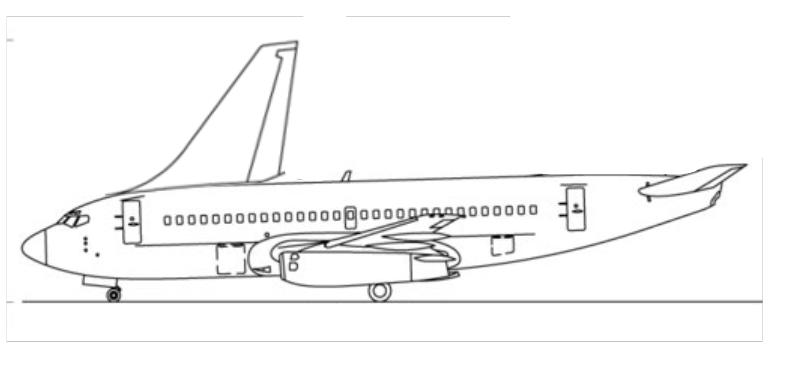
\includegraphics[width=0.65\textwidth]{ForwardVStab.png}
        % \caption{}
        % \label{fig:enter-label}
    \end{figure}
    \begin{enumerate}
        \item Re-derive the yaw stiffness contribution from the vertical stabilizer, $C_{{n_F}_\beta} = \frac{\partial C_{{n_F}}}{\partial \beta}$. Let the sidewash angle, $\sigma$, and $\frac{\partial \sigma}{\partial \beta}$ be 0. Thus, $\alpha_F = -\beta$. What is the sign of $C_{{n_F}_\beta}$?
        \item Re-derive the ``rudder power" $C_{n_{\delta_r}}$.
        \item Is this a good aircraft design? Why or why not?
    \end{enumerate}
\end{question}

\vspace{0.1cm}

\clearpage

\begin{question}
    While flying near sea-level at $u_0 = 10$ m/s, the TTwistor aircraft from homework P3 has the lateral dynamics matrix shown below.
    \begin{align*}
        \mathbf{A}_{lat} = 
        \begin{bmatrix}
         -0.2472 & -0.0671 & -9.7797 & 9.8100 \\
         -0.7966 & -16.5375 & 1.8114 & 0 \\
         0.4607 & -0.3451 & -0.4586 &  0 \\
         0 & 1.0000 & 0 & 0
        \end{bmatrix}
    \end{align*}
    Assume for this analysis that the aircraft's inertia matrix is diagonal, so that only $I_x$, $I_y$, and $I_z$ are non-zero. This means that $\Gamma_3 = 1/I_x$, $\Gamma_4 = 0$, and $\Gamma_8 = 1/I_z$.
    
    \begin{enumerate}
        \item Calculate the time constant ($\tau_{roll} = 1/|\lambda|$) of the roll mode and the natural frequency $\omega_{n,dr}$ of the Dutch roll mode.
        \item Recall that nine lateral dimensional stability derivatives appear in the expression for $\mathbf{A}_{lat}$. One-by-one, increase the value of each dimensional stability derivative by 10\% and calculate the new time constant of the roll mode and new natural frequency of the dutch roll mode. So, first, increase $Y_v$ by 10\% and calculate the new values of $\tau_{roll}$ and $\omega_{n,dr}$. Then, return $Y_v$ to its original value and increase the next stability derivative by 10\%. You do not need to report every value that you calculate, but do answer the following:
        \begin{enumerate}
            \item A change in which stability derivative decreases the time constant of the roll mode the most? What is the new time constant when this derivative is increased by 10\%?
            \item A change in which stability derivative increases the natural frequency of the Dutch roll mode the most? What is the new natural frequency when this derivative is increased by 10\%?
        \end{enumerate}
        \item Qualitatively explain why the two stability derivatives you identified in the previous part have the largest effect on $\tau_{roll}$ and $\omega_{n,dr}$ using characteristics of the roll and Dutch roll modes.
    \end{enumerate}
\end{question}
\vspace{0.1cm}

\end{document}
